\documentclass[14pt,a4paper]{extarticle}
\usepackage[T2A]{fontenc}
\usepackage[utf8]{inputenc}
\usepackage[english,russian]{babel}
\usepackage{lmodern}
\usepackage{geometry}
\usepackage{array}
\usepackage{tabularx}
\usepackage{longtable}
\usepackage{ltablex}
\usepackage{booktabs}
\usepackage{hyperref}
\usepackage{indentfirst}
\usepackage{microtype}
\usepackage{graphicx}
\usepackage{setspace}
\usepackage{listings}
\usepackage{graphicx}
\usepackage{caption}
\usepackage{float}
\usepackage{tocloft}
\usepackage{titlesec}
\usepackage{newtxtext,newtxmath}
\usepackage{eqexpl}
\usepackage{minted}
\usepackage{totcount}
\usepackage{lastpage}

\newcommand{\R}{\ensuremath{\mathbb{R}}}

\titleformat{\section}        % форматируем \section
  {\normalfont\bfseries}      % стиль: обычный + жирный
  {\thesection.}              % номер секции с точкой
  {2mm}                       % расстояние между номером и текстом
  {}                           % перед заголовком можно добавить что-то
\titlespacing*{\section}{1.5cm}{*3}{*1}  % {отступ слева}{отступ сверху}{отступ снизу}

\titleformat{\subsection}        % форматируем \section
  {\normalfont\bfseries}      % стиль: обычный + жирный
  {\thesubsection.}              % номер секции с точкой
  {2mm}                       % расстояние между номером и текстом
  {}                           % перед заголовком можно добавить что-то
\titlespacing*{\subsection}{1.5cm}{*3}{*1}  % {отступ слева}{отступ сверху}{отступ снизу}

\captionsetup{justification=centering}
\renewcommand{\ttdefault}{cmtt}
\keepXColumns
\setlength{\parindent}{3em}
\newgeometry{left=2.5cm,right=2.5cm,top=3cm,bottom=2.5cm}

\renewcommand{\contentsname}{\hspace*{4em}{\smallСодержание}}
\setlength{\cftbeforesecskip}{0.5em}
\renewcommand{\cftsecleader}{\cftdotfill{\cftdotsep}}
\renewcommand{\cftsecaftersnum}{.\hspace{2mm}}

% counters
\regtotcounter{figure}
\regtotcounter{table}
\regtotcounter{page}

\title{Отчёт по Машинному обучению}
\author{Выполнил студент группы М-РИТ-25-1, Станиславчук Сергей}

\begin{document}

\setstretch{1.5}
\noindent
\begin{minipage}[t]{0.01\textwidth}
    \includegraphics{~/programmer/++Programmer/5_1/LSTU.jpg}
\end{minipage}%
\begin{minipage}[c]{1.1\linewidth}
    \centering
    {\small
    МИНИСТЕРСТВО НАУКИ И ВЫСШЕГО ОБРАЗОВАНИЯ РФ \\[1em]
    ФЕДЕРАЛЬНОЕ ГОСУДАРСТВЕННОЕ БЮДЖЕТНОЕ \\
    ОБРАЗОВАТЕЛЬНОЕ УЧРЕЖДЕНИЕ ВЫСШЕГО ОБРАЗОВАНИЯ \\
    «ЛИПЕЦКИЙ ГОСУДАРСТВЕННЫЙ ТЕХНИЧЕСКИЙ УНИВЕРСИТЕТ»
    }
\end{minipage}%

\vspace{3em}

\noindent
\hspace{1em}%
\begin{minipage}[t]{0.8\textwidth}
\textbf{Институт} \hspace{2em} компьютерных наук \\
\textbf{Кафедра} \hspace{2em} автоматизированных систем управления
\end{minipage}

\vspace{6em}

\begin{center}
    Курсовая работа \\
    по дисциплине: <<Техологии обработки больших массивов данных>>
    Проектирование системы обработки больших массивов данных
\end{center}

\vspace{6em}

\noindent
\begin{tabular*}{\textwidth}{@{\extracolsep{\fill}} l c r }
    Студент М-РИТ-25-1 & \makebox[4cm]{\hrulefill} & Станиславчук С.М. \\[2em]
Руководитель & \\
Доцент, к.т.н. & \makebox[4cm]{\hrulefill} & Тюрин А.С. \\
\end{tabular*}

\vfill
\begin{center}
    Липецк, 2025
\end{center}

\thispagestyle{empty}

\newpage
\tableofcontents
\newpage

\section{Аннотация}
\begin{sloppypar}
    С.~\pageref{LastPage}, Ил. \total{figure}, Литература 5 назв.

В данной курсовой работе приводится описание используемых средств,
    проектируется система обработки и анализа больших массивов данных,
    реализуется графический вывод информации, а также оповещение
    заинтересованных лиц о состоянии системы.
\end{sloppypar}

\newpage
\section{Задание кафедры}

Спроектировать шаблон системы обработки и анализа больших, описать используемые
для этого средства, привести примеры графиков из систем мониторинга, добавить
оповещение об превышении нормальных значений определенных параметров системы.


\newpage
\section{Docker}
Docker — это программная платформа для автоматизированного развёртывания и
управления приложениями с использованием контейнерной технологии. Она позволяет
упаковать приложение вместе со всеми зависимостями и окружением в изолированный
контейнер, который можно запускать на любой Linux-системе с поддержкой cgroups.
Docker также предоставляет удобный набор команд для управления такими
контейнерами. Изначально технология базировалась на LXC, однако с 2015 года
используется собственная библиотека libcontainer, абстрагирующая механизмы
виртуализации ядра Linux. С созданием Open Container Initiative архитектура
Docker начала эволюционировать от монолитной к модульной.

Проект разрабатывается и поддерживается одноимённой компанией и
распространяется в двух вариантах: открытая версия Community Edition под
лицензией Apache 2.0 и корпоративная Enterprise Edition с проприетарной
лицензией. Реализован Docker на языке Go.

Docker работает в среде Linux с ядром, поддерживающим контрольные группы и
пространства имён (namespaces). Доступны сборки для архитектур x86-64 и ARM, а
начиная с версии 1.6 (апрель 2015 года) появилась возможность использования
Docker в операционных системах семейства Windows.

Для эффективного использования дискового пространства Docker применяет файловую
систему Aufs с поддержкой объединённого монтирования: контейнеры используют
общий базовый образ операционной системы, а все изменения сохраняются отдельно.
Также поддерживается использование файловой системы Btrfs с механизмом
copy-on-write.

В состав Docker входит демон — сервер контейнеров, клиентские утилиты командной
строки для управления образами и контейнерами, а также REST-подобный API,
позволяющий управлять контейнерами программно. Демон обеспечивает изоляцию
контейнеров на уровне файловой системы, процессов и сети, гарантируя
независимость их работы и распределение ресурсов средствами libcontainer.

Клиентские инструменты позволяют запускать, останавливать, перезапускать,
приостанавливать и возобновлять контейнеры, а также отслеживать их состояние и
выполняемые процессы. Образы могут создаваться на основе сценариев Dockerfile
или формироваться из текущего состояния контейнера. Все команды могут
взаимодействовать как с локальным Docker-демоном, так и с удалёнными серверами.
Кроме того, Docker интегрирован с публичным репозиторием Docker Hub, где можно
искать, загружать и публиковать образы приложений.

Дополнительно Docker включает инструмент Docker Compose — средство для описания
и запуска многоконтейнерных приложений. Конфигурации Compose задаются в файлах
формата YAML и позволяют централизованно управлять сложными сервисными
структурами.

\newpage
\section{Docker Compose}
Docker Compose — это инструмент для управления несколькими контейнерами,
работающими как единое приложение. Он особенно полезен при микросервисной
архитектуре, когда приложение состоит из набора независимых сервисов,
взаимодействующих между собой по сети, чаще всего через HTTP-запросы.

По сути, Docker Compose расширяет возможности Docker, упрощая работу со
сложными конфигурациями. Даже в сценариях с одним контейнером Compose даёт
преимущество — конфигурация приложения становится декларативной и независимой
от конкретных команд запуска, чего нельзя добиться с помощью одного лишь
Dockerfile. Все параметры, включая проброс портов, подключение томов и
переменные окружения, описываются в файле `docker-compose.yml`.

На рисунке \ref{fig:dc1} представлен интерфейс командной строки docker-compose, где
выполняется загрузка изображений контейнеров <<Spark>>.

\begin{figure}[H]
    \centering
    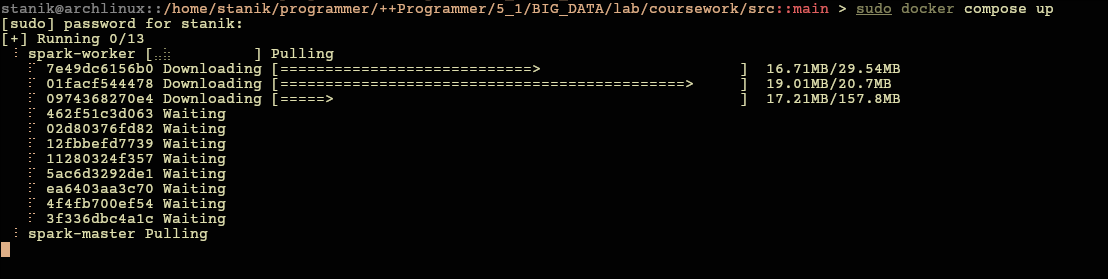
\includegraphics[width=0.78\textwidth]{pic2.png}
    \refstepcounter{figure}
    \caption*{Рисунок \thefigure\ — CLI Docker Compose загрузка}
    \label{fig:dc1}
\end{figure}

На рисунке \ref{fig:dc2} представлен интерфейс командной строки docker-compose, где
выполняется запуск контейнеров с указанием режима "detached".

\begin{figure}[H]
    \centering
    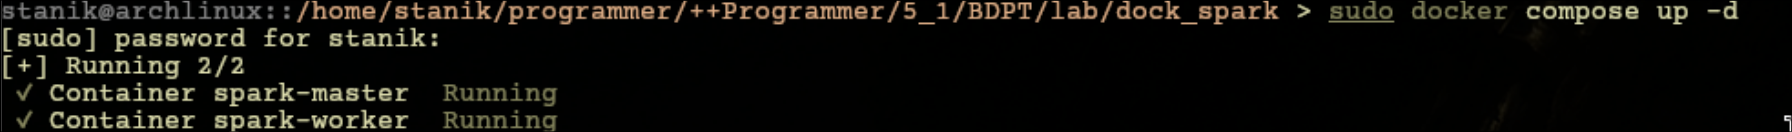
\includegraphics[width=0.78\textwidth]{pic1.png}
    \refstepcounter{figure}
    \caption*{Рисунок \thefigure\ — CLI Docker Compose запуск}
    \label{fig:dc2}
\end{figure}

\newpage
\section{Spark}

Apache Spark — это распределённая платформа для обработки больших массивов
данных, ориентированная на высокую производительность и масштабируемость. Она
предназначена для выполнения вычислений в кластере и поддерживает как пакетную,
так и потоковую обработку данных. Благодаря архитектуре, основанной на
обработке данных в оперативной памяти, Spark значительно превосходит
традиционные MapReduce-подходы по скорости выполнения аналитических задач.

Платформа предоставляет унифицированную модель программирования и набор
высокоуровневых API для языков Scala, Java, Python и R. Это позволяет
использовать Spark для решения широкого круга задач: анализа данных, машинного
обучения, потоковой обработки, построения графов и SQL-запросов к
распределённым наборам данных. Центральным элементом вычислительной модели
Spark являются RDD, DataFrame и Dataset, обеспечивающие отказоустойчивость и
параллельную обработку.

Apache Spark органично интегрируется с экосистемой Hadoop и может использовать
HDFS в качестве распределённого хранилища данных. При этом Spark не требует
обязательного использования Hadoop YARN и может работать в автономном режиме
либо под управлением внешних менеджеров ресурсов. Поддержка Apache Kafka делает
Spark удобным инструментом для построения конвейеров потоковой обработки данных
в реальном времени.

Благодаря модульной архитектуре Spark широко применяется в системах обработки
больших данных, где требуется сочетание высокой скорости обработки, гибкости и
интеграции с другими компонентами распределённой инфраструктуры. Это делает его
ключевым элементом современных аналитических платформ в научных, коммерческих и
инженерных проектах.

\subsection{Архитектура}

Архитектура Apache Spark основана на модели «ведущий–исполнитель», которая
обеспечивает централизованное управление вычислительными ресурсами и
параллельное выполнение задач. В рамках данной модели ключевыми компонентами
являются Spark Master и Spark Worker, каждый из которых выполняет строго
определённые функции в распределённой системе обработки данных.

Spark Master выступает в роли управляющего узла кластера. Он отвечает за приём
и распределение вычислительных задач между рабочими узлами, а также за
управление доступными ресурсами кластера, такими как процессорное время и
оперативная память. Master отслеживает состояние подключённых рабочих узлов,
принимает решения о запуске приложений и обеспечивает координацию их
выполнения. Таким образом, Spark Master не участвует непосредственно в
обработке данных, а выполняет функции диспетчера и координатора вычислений.

Spark Worker представляет собой исполнительный узел, на котором непосредственно
выполняются вычислительные задачи. Каждый Worker предоставляет кластеру
определённый объём ресурсов и запускает один или несколько executor-процессов
Spark. Именно executors обрабатывают данные, выполняют преобразования и
действия, а также взаимодействуют с внешними источниками и хранилищами данных,
такими как HDFS или Kafka. Наличие нескольких Worker-узлов позволяет
распределять нагрузку и масштабировать систему горизонтально за счёт добавления
новых узлов без изменения логики приложений.

Разделение функций управления и исполнения повышает отказоустойчивость и
производительность системы. При увеличении объёма данных или вычислительной
нагрузки достаточно добавить новые Worker-контейнеры, в то время как Master
продолжает выполнять функции координации без необходимости переработки
архитектуры.

К сожалению, с недавних пор, образ \texttt{bitnami/spark} более недоступен бесплатно.
Все его версии были убраны с \texttt{Docker Hub}. Поэтому в данной работе будет использоваться
образ \texttt{apache/spark}.

Для того чтобы запустить контейнер <<Spark Master>>, нужно добавить следующий кусок кода в
\texttt{docker\_compose.yml} в раздел <<services>>

\begin{verbatim}

  spark-master:
    image: apache/spark:latest
    container_name: spark-master
# для инициализации контейнера как мастер
    command: >
      /opt/spark/bin/spark-class
      org.apache.spark.deploy.master.Master
    ports:
      - "7077:7077" # рабочий порт
      - "8080:8080" # WebUI
    networks:
      - spark-net   # общий network с воркером

\end{verbatim}

Параметр container\_name задаёт фиксированное имя контейнера, что упрощает
сетевое взаимодействие между компонентами кластера и облегчает обращение к
Spark Master из других сервисов. Директива command переопределяет команду
запуска контейнера и используется для инициализации Spark в режиме управляющего
узла (Master) путём запуска класса org.apache.spark.deploy.master.Master.

В разделе ports выполняется проброс основных портов Spark Master на хостовую
систему. Порт 7077 используется для взаимодействия с рабочими узлами (Spark
Worker) и для приёма заданий, отправляемых с помощью утилиты spark-submit. Порт
8080 предназначен для доступа к веб-интерфейсу Spark, который позволяет
отслеживать состояние кластера, запущенные приложения и распределение ресурсов.

Параметр networks указывает на подключение контейнера к общей Docker-сети
spark-net, обеспечивая сетевую связность Spark Master с рабочими узлами, а
также с другими компонентами системы, использующими вычислительные ресурсы
Spark.

Для того чтобы запустить контейнер <<Spark Worker>>, нужно добавить следующий кусок кода в
\texttt{docker\_compose.yml} в раздел <<services>>:

\begin{verbatim}

  spark-worker:
    container_name: spark-worker
    # для инициализации контейнера как воркер
    command: >
      /opt/spark/bin/spark-class
      org.apache.spark.deploy.worker.Worker
# адрес для обращения к мастеру
      spark://spark-master:7077
# контейнер не будет запущен, пока spark-master не закончит запуск удачно
    depends_on:
      - spark-master
    ports:
      - "8081:8081"
    networks:
      - spark-net # общий network с мастером

\end{verbatim}
Параметр container\_name задаёт фиксированное имя контейнера, что упрощает его
идентификацию и сетевое взаимодействие с управляющим узлом кластера. Директива
command переопределяет стандартную команду запуска контейнера и используется
для инициализации Spark в режиме рабочего узла (Worker) путём запуска класса
org.apache.spark.deploy.worker.Worker. В качестве аргумента указывается адрес
Spark Master (spark://spark-master:7077), по которому рабочий узел
регистрируется в кластере и получает задания на выполнение.

Параметр depends\_on определяет зависимость запуска контейнера от сервиса Spark
Master и гарантирует, что рабочий узел будет запущен только после успешной
инициализации управляющего узла. Это предотвращает ошибки подключения и
обеспечивает корректную регистрацию Worker в кластере.

В разделе ports выполняется проброс порта 8081, который используется для
доступа к веб-интерфейсу Spark Worker. Данный интерфейс позволяет отслеживать
состояние рабочего узла, активные задачи и использование вычислительных
ресурсов. Параметр networks указывает на подключение контейнера к общей
Docker-сети spark-net, обеспечивая сетевую связность Spark Worker с управляющим
узлом и другими компонентами распределённой системы.

Веб-интерфейс (WebUI) работающего Spark Master представлен на рисунке ~\ref{fig:spm}.

\begin{figure}[H]
    \centering
    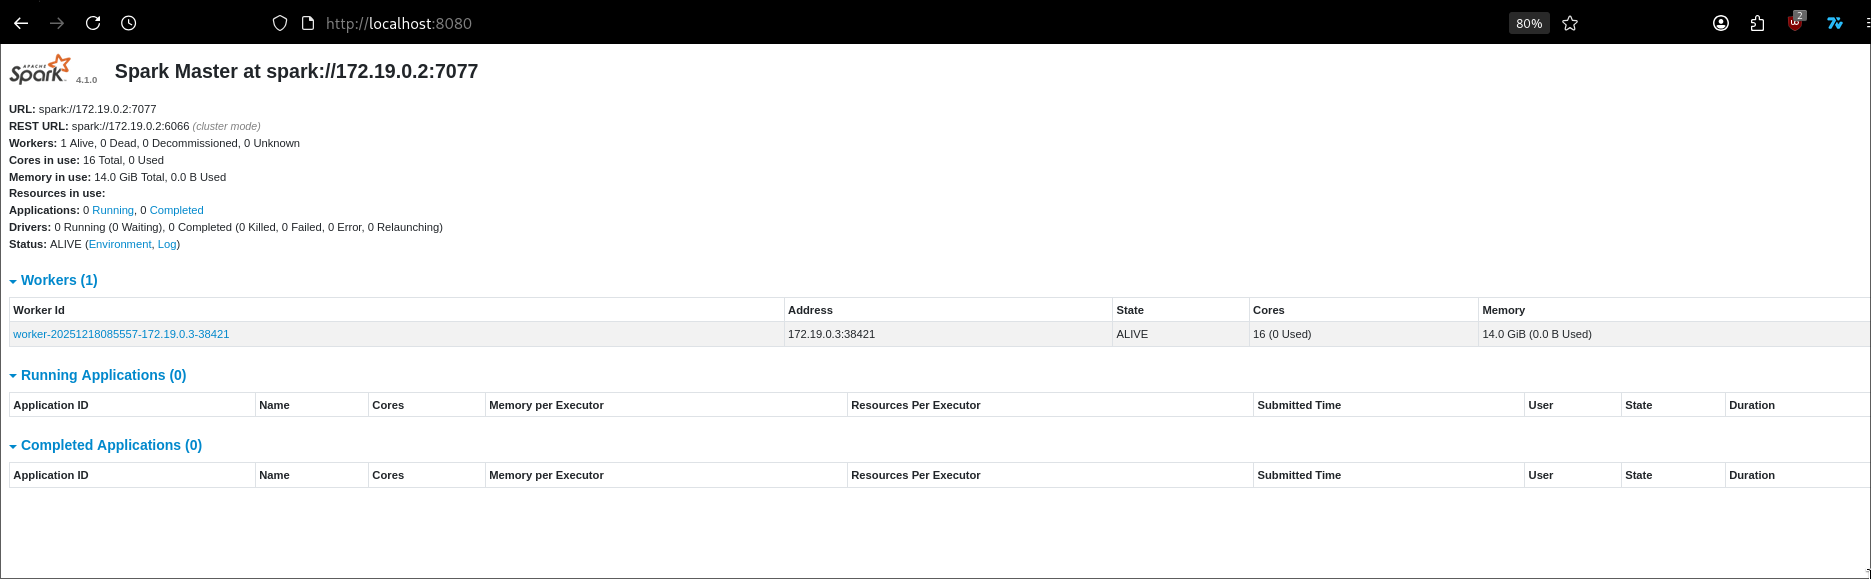
\includegraphics[width=0.78\textwidth]{sparkm.png}
    \refstepcounter{figure}
    \caption*{Рисунок \thefigure\ — Spark Master}
    \label{fig:spm}
\end{figure}


\newpage
\section{Apache Kafka}

Apache Kafka — это распределённая платформа потоковой передачи данных,
предназначенная для надёжного и высокопроизводительного обмена сообщениями
между компонентами распределённых информационных систем. Kafka используется для
организации асинхронного взаимодействия между источниками данных и системами их
обработки, обеспечивая устойчивую передачу больших объёмов событий в режиме,
близком к реальному времени.

Основу архитектуры Kafka составляет модель публикации–подписки, в рамках
которой производители данных (producers) публикуют сообщения в логически
организованные каналы — топики, а потребители (consumers) считывают эти
сообщения независимо друг от друга. Сообщения внутри топиков хранятся в
упорядоченном виде и распределяются по партициям, что позволяет масштабировать
систему горизонтально и обрабатывать потоки данных параллельно.

Kafka обеспечивает высокую отказоустойчивость за счёт репликации данных между
узлами кластера и сохраняет сообщения на диске в течение заданного времени,
независимо от скорости их потребления. Благодаря этому платформа может
использоваться не только как транспорт событий, но и как временное хранилище
потоковых данных. В экосистемах обработки больших данных Kafka часто выступает
связующим звеном между системами сбора данных и аналитическими платформами,
такими как Apache Spark.

В контексте данной курсовой работы Kafka применяется в роли источника потоковых
данных для системы аналитической обработки. Она обеспечивает поступление данных
в реальном времени, которые далее передаются в Apache Spark для обработки и
последующего сохранения в распределённом хранилище Hadoop или визуализации
агрегированных метрик.

Для работы Kafka требуется 2 компонента: брокер Kafka и сервис координации. В
качестве сервиса координации будет использован Apache ZooKeeper.

Для того чтобы запустить контейнер <<Apache Kafka>>, нужно добавить следующий
блок текста в конфигурационный файл \texttt{docker\_compose.yml} в раздел
<<services>>:

\begin{verbatim}

  kafka:
    image: confluentinc/cp-kafka:7.0.1
    depends_on:
      - zookeeper
    ports:
      - "9092:9092"
      - "29092:29092"
    environment:
      KAFKA_BROKER_ID: 1
      KAFKA_ZOOKEEPER_CONNECT: zookeeper:2181
      KAFKA_ADVERTISED_LISTENERS: PLAINTEXT://kafka:29092,PLAINTEXT_HOST://localhost:9092
      KAFKA_LISTENER_SECURITY_PROTOCOL_MAP: PLAINTEXT:PLAINTEXT,PLAINTEXT_HOST:PLAINTEXT
      KAFKA_INTER_BROKER_LISTENER_NAME: PLAINTEXT
      KAFKA_OFFSETS_TOPIC_REPLICATION_FACTOR: 1
    network:
        spark-net

\end{verbatim}

В разделе environment задаются основные параметры работы ZooKeeper. Переменная
ZOOKEEPER\_CLIENT\_PORT определяет порт, на котором сервис принимает клиентские
подключения, что необходимо для взаимодействия с брокером Kafka. Параметр
ZOOKEEPER\_TICK\_TIME задаёт базовый временной интервал в миллисекундах,
используемый ZooKeeper для внутренних механизмов синхронизации и управления
сессиями.

Директива ports выполняет проброс клиентского порта ZooKeeper на хостовую
систему, что позволяет другим компонентам системы и средствам отладки
обращаться к сервису извне контейнерной среды. Параметр network указывает на
использование общей Docker-сети spark-net, обеспечивая сетевую связность
ZooKeeper с другими сервисами распределённой системы, включая брокер Kafka.

Параметр \texttt{KAFKA\_CFG\_LISTENERS} отвечает за то, на каком адресе Kafka слушает подключения.
Параметр \texttt{KAFKA\_CFG\_ADVERTISED\_LISTENERS} отвечает за то, какой адрес Kafka сообщает клиентам.

Для того чтобы запустить контейнер <<Apache ZooKeeper>>, нужно добавить
следующий блок текста в конфигурационный файл \texttt{docker\_compose.yml} в
раздел <<services>>:

\begin{verbatim}

  zookeeper:
    image: confluentinc/cp-zookeeper:7.0.1
    environment:
      ZOOKEEPER_CLIENT_PORT: 2181
      ZOOKEEPER_TICK_TIME: 2000
    ports:
      - "2181:2181"
    network:
        spark-net

\end{verbatim}

Для того чтобы запустить контейнер <<Kafdrop>>, нужно добавить
следующий блок текста в конфигурационный файл \texttt{docker\_compose.yml} в
раздел <<services>>:

\begin{verbatim}

  kafdrop:
    image: obsidiandynamics/kafdrop:latest
    depends_on:
      - kafka
    ports:
      - "9000:9000"
    environment:
      KAFKA_BROKER_CONNECT: kafka:29092
      JVM_OPTS: "-Xms32M -Xmx64M"
      SERVER_SERVLET_CONTEXTPATH: "/"

\end{verbatim}

Директива ports выполняет проброс порта контейнера на хостовую систему, что
позволяет получить доступ к веб-интерфейсу Kafdrop через браузер по адресу
http://localhost:9000. В переменной окружения KAFKA\_BROKER\_CONNECT задаётся
адрес брокера Kafka, к которому Kafdrop подключается для получения информации о
топиках, партициях и сообщениях. Параметр JVM\_OPTS используется для ограничения
объёма оперативной памяти, выделяемой виртуальной машине Java, что снижает
потребление ресурсов контейнером. Параметр SERVER\_SERVLET\_CONTEXTPATH задаёт
корневой контекст веб-приложения, обеспечивая доступ к интерфейсу без
дополнительного префикса в URL.

На рисунке \ref{fig:kafdrop} представлен WebUI Kafdrop.

\begin{figure}[H]
    \centering
    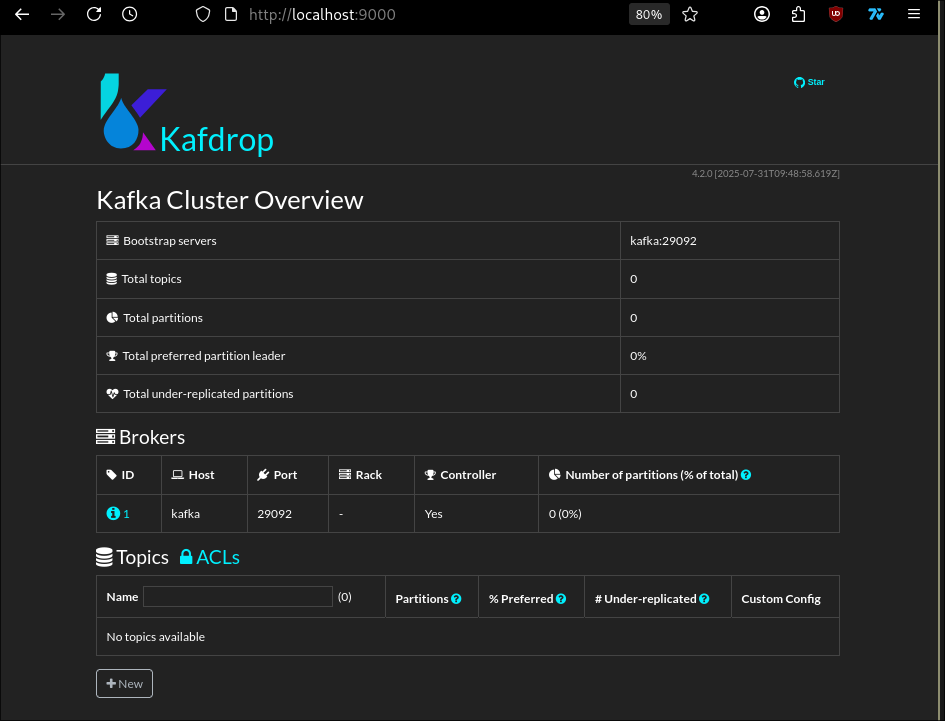
\includegraphics[width=0.78\textwidth]{kafdrop.png}
    \refstepcounter{figure}
    \caption*{Рисунок \thefigure\ — WebUI кафдроп}
    \label{fig:kafdrop}
\end{figure}


\newpage
\section{Node exporter}
Для сбора системных метрик вычислительных узлов в работе использован Prometheus
Node Exporter. Данный компонент предназначен для мониторинга состояния
операционной системы и аппаратных ресурсов узла, включая загрузку центрального
процессора, использование оперативной памяти, дисковой подсистемы и сетевых
интерфейсов. Node Exporter функционирует как источник метрик для Prometheus и
позволяет получать объективную информацию о фактической нагрузке на хост и
контейнеры, на которых выполняются компоненты распределённой системы.

Использование Node Exporter в связке с Prometheus и Grafana обеспечивает
низкоуровневое наблюдение за состоянием вычислительной инфраструктуры и
дополняет прикладные метрики Apache Spark, что позволяет проводить комплексный
анализ производительности системы и выявлять узкие места как на уровне
приложений, так и на уровне операционной среды.

\section{Zookeeper}
Apache ZooKeeper используется в системе как распределённый сервис координации,
обеспечивающий согласованную работу компонентов Apache Kafka. ZooKeeper
отвечает за хранение и синхронизацию метаданных кластера, включая информацию о
брокерах, топиках, партициях и лидерах реплик, а также за выполнение механизмов
выбора лидера и обнаружения отказов. Благодаря использованию ZooKeeper
обеспечивается отказоустойчивость и согласованность работы Kafka в
распределённой среде, что является критически важным для корректной обработки и
доставки потоковых данных.

\section{Spark Exporter}
Spark Exporter применяется для интеграции Apache Spark с системой мониторинга
Prometheus. Данный компонент осуществляет сбор метрик из Spark через интерфейс
JMX и преобразует их в формат, совместимый с Prometheus. Экспортер
предоставляет информацию о состоянии Spark-приложений, работе исполнителей
(executors), использовании вычислительных ресурсов, активности задач и
параметрах виртуальной машины Java. Использование Spark Exporter позволяет
получать детализированные метрики производительности Spark и визуализировать их
в Grafana, что способствует анализу эффективности распределённых вычислений и
своевременному выявлению проблем в работе кластера.

\newpage
\section{Apache Hadoop}
Apache Hadoop — это распределённая платформа для хранения и обработки больших
объёмов данных, разработанная для обеспечения масштабируемости,
отказоустойчивости и высокой производительности при работе с массивными
наборами информации. Hadoop позволяет распределять данные по множеству узлов
кластера и выполнять вычисления параллельно, что делает его ключевым
компонентом экосистемы больших данных.

Центральной частью Hadoop является распределённая файловая система HDFS (Hadoop
Distributed File System), которая обеспечивает надёжное хранение данных, их
репликацию и доступность даже в случае выхода из строя отдельных узлов. HDFS
разбивает файлы на блоки, которые распределяются по узлам кластера, и хранит
несколько копий каждого блока, обеспечивая устойчивость к сбоям.

Для обработки данных в Hadoop используется модель MapReduce, позволяющая
выполнять вычисления в параллельном режиме непосредственно на узлах, где
хранятся данные, что минимизирует передачу информации по сети. Благодаря этому
Hadoop эффективен при работе с большими объёмами информации и сложными
аналитическими задачами.

Hadoop также является платформой интеграции с другими компонентами экосистемы
обработки данных. В частности, Apache Spark может использовать HDFS как
источник и хранилище данных, получая возможность выполнять
высокопроизводительную обработку, а системы потоковой передачи, такие как
Kafka, могут передавать данные в HDFS через Spark Streaming. Такой подход
позволяет строить конвейеры обработки данных в реальном времени и пакетные
аналитические процессы в единой инфраструктуре.

В рамках данной курсовой работы Hadoop выступает в качестве распределённого
хранилища для накопления и последующей аналитической обработки больших потоков
данных, обеспечивая надёжность, масштабируемость и интеграцию с компонентами
Spark и Kafka.


Для того чтобы запустить контейнер <<Apache Hadoop>>, нужно добавить
следующий блок текста в конфигурационный файл \texttt{docker\_compose.yml} в
раздел <<services>>:

\begin{verbatim}

  namenode:
    image: bde2020/hadoop-namenode:2.0.0-hadoop3.2.1-java8
    container_name: namenode
    hostname: namenode
    ports:
      - "9870:9870"  # Web UI
      - "9000:9000"  # RPC port
    environment:
      - CLUSTER_NAME=hadoop-cluster
      - CORE_CONF_fs_defaultFS=hdfs://namenode:9000
    volumes:
      - namenode-data:/hadoop/dfs/name
    restart: unless-stopped

  datanode1:
    image: bde2020/hadoop-datanode:2.0.0-hadoop3.2.1-java8
    container_name: datanode1
    hostname: datanode1
    environment:
      - CORE_CONF_fs_defaultFS=hdfs://namenode:9000
      - HDFS_CONF_dfs__client__use__datanode__hostname=false
    ports:
      - "9864:9864"
    volumes:
      - datanode1-data:/hadoop/dfs/data
    depends_on:
      - namenode
    restart: unless-stopped

  datanode2:
    image: bde2020/hadoop-datanode:2.0.0-hadoop3.2.1-java8
    container_name: datanode2
    hostname: datanode2
    environment:
      - CORE_CONF_fs_defaultFS=hdfs://namenode:9000
      - HDFS_CONF_dfs__client__use__datanode__hostname=false
    volumes:
      - datanode2-data:/hadoop/dfs/data
    depends_on:
      - namenode
    ports:
      - "9865:9864"
    restart: unless-stopped

\end{verbatim}

WebUI Apache Hadoop для <<namenode>> изображен на рисунке \ref{fig:namenode}

\begin{figure}[H]
    \centering
    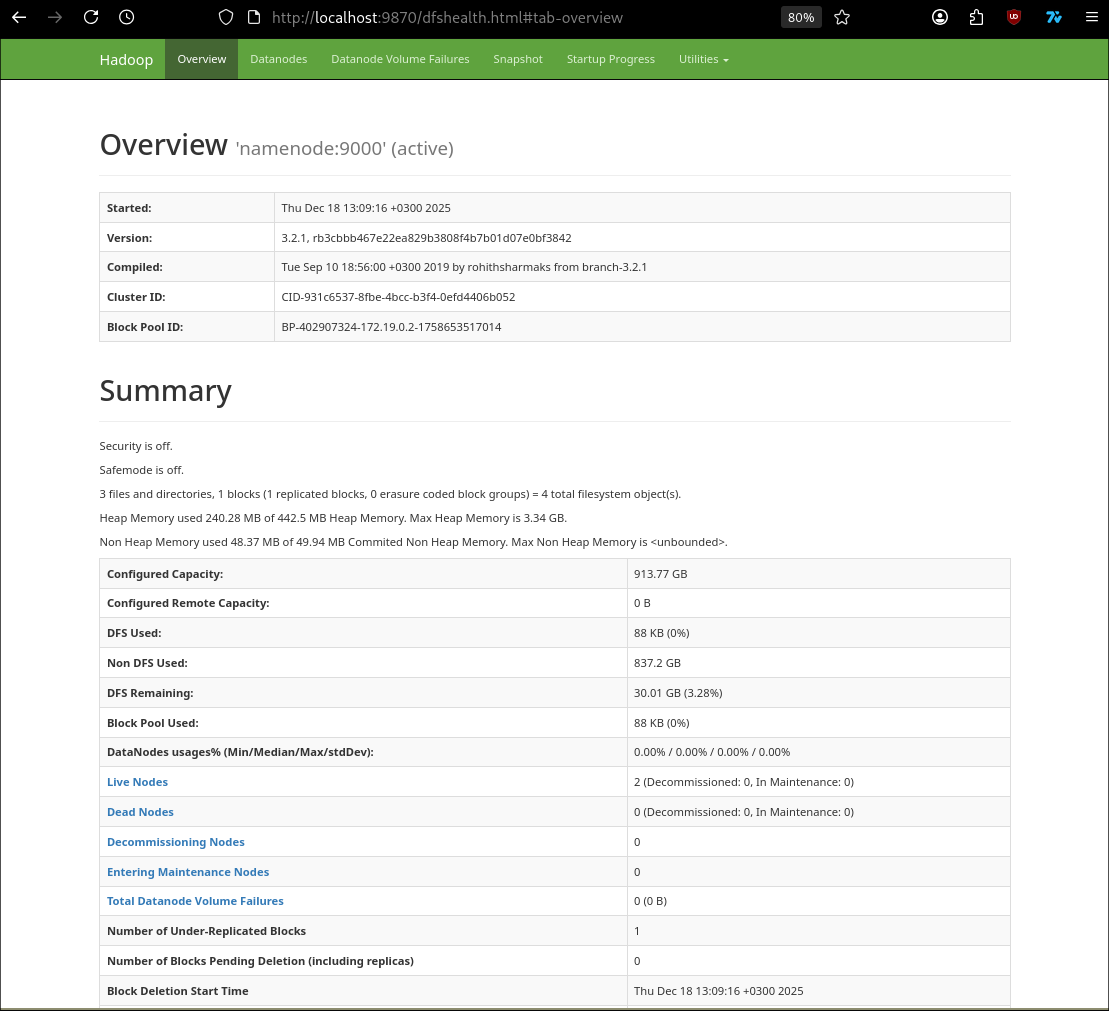
\includegraphics[width=0.78\textwidth]{namenode.png}
    \refstepcounter{figure}
    \caption*{Рисунок \thefigure\ — WebUI неймноды}
    \label{fig:namenode}
\end{figure}

\newpage
\section{Grafana}

Grafana — это платформа для визуализации и мониторинга данных, предназначенная
для создания интерактивных дашбордов и аналитических панелей в реальном
времени. Она позволяет собирать метрики из различных источников, включая базы
данных, системы мониторинга и потоки событий, и представлять их в удобной
графической форме.

Одним из ключевых преимуществ Grafana является возможность подключения к
разнообразным источникам данных, таким как Prometheus, InfluxDB, Elasticsearch,
PostgreSQL и другие, включая метрики приложений и системные показатели. Это
делает Grafana универсальным инструментом для наблюдения за состоянием
распределённых систем и анализа производительности.

В контексте обработки больших массивов данных Grafana используется для
визуализации результатов работы аналитических конвейеров, таких как Apache
Spark, а также мониторинга потоков данных из Apache Kafka. Это позволяет в
реальном времени отслеживать нагрузку на систему, скорость обработки сообщений,
состояние кластеров и другие ключевые показатели, обеспечивая возможность
принятия своевременных и обоснованных решений.

Контейнеризация Grafana позволяет быстро разворачивать платформу и
интегрировать её с остальными компонентами системы обработки данных. Через
веб-интерфейс пользователи могут создавать кастомные дашборды, строить графики
и таблицы, настраивать оповещения и агрегировать метрики из различных
источников, что делает Grafana важным инструментом визуальной аналитики в
современных экосистемах больших данных.

В рамках курсовой работы Grafana выполняет роль визуального слоя, обеспечивая
наблюдение за состоянием потоков данных и вычислительных процессов, поступающих
из Kafka и обрабатываемых Spark, а также контролируя метрики распределённого
хранилища Hadoop.

\newpage
\section{Демонстрация работы системы}

Для того, чтобы визуализировать метрики spark-worker в Grafana, нужно добавить spark-exporter в Prometheus (как новый scrape).

Prometheus.yml (добавление spark-exporter):

\begin{verbatim}

  - job_name: 'spark'
    static_configs:
      - targets: ['spark-exporter:9091']

\end{verbatim}

Теперь посылаем метрики из Spark в Kafka и смотрим результат в отдельном топике через KafDrop

В качестве тестового бенчмарка, буду использовать встроенный SparkPi:

\begin{verbatim}

/opt/spark/bin/spark-submit \
  --master spark://spark-master:7077 \
  --class org.apache.spark.examples.SparkPi \
  /opt/spark/examples/jars/spark-examples_*.jar \
  100000

\end{verbatim}

Часть логов выполнения задач из цикла размером 10000, изображена на рисунке \ref{fig:logs-cycle}

\begin{figure}[H]
    \centering
    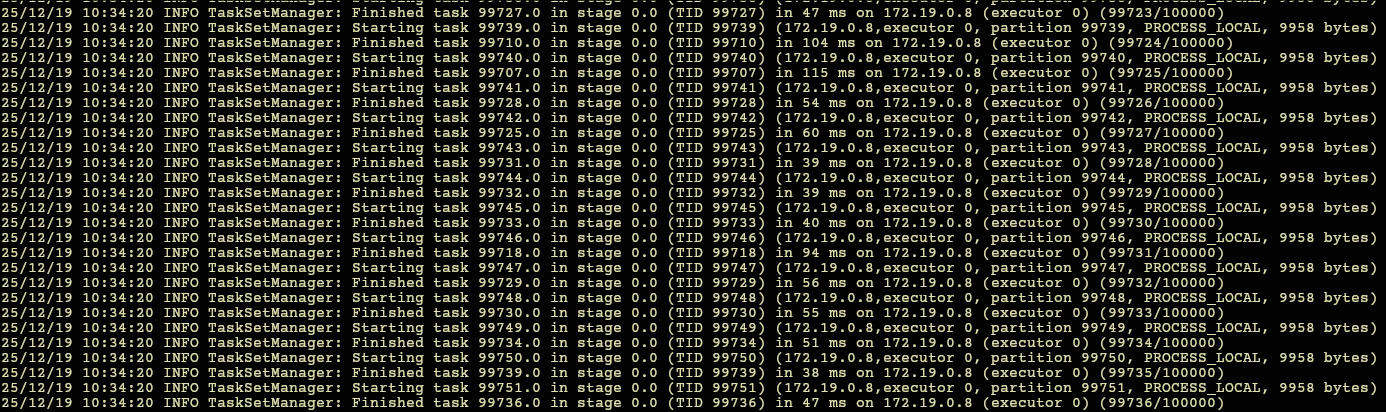
\includegraphics[width=0.78\textwidth]{logs-cycle.png}
    \refstepcounter{figure}
    \caption*{Рисунок \thefigure\ — метрики Spark воркера}
    \label{fig:logs-cycle}
\end{figure}


Мастер, передающий цикл задач воркеру, изображен на рисунке \ref{fig:spark_master_running}

\begin{figure}[H]
    \centering
    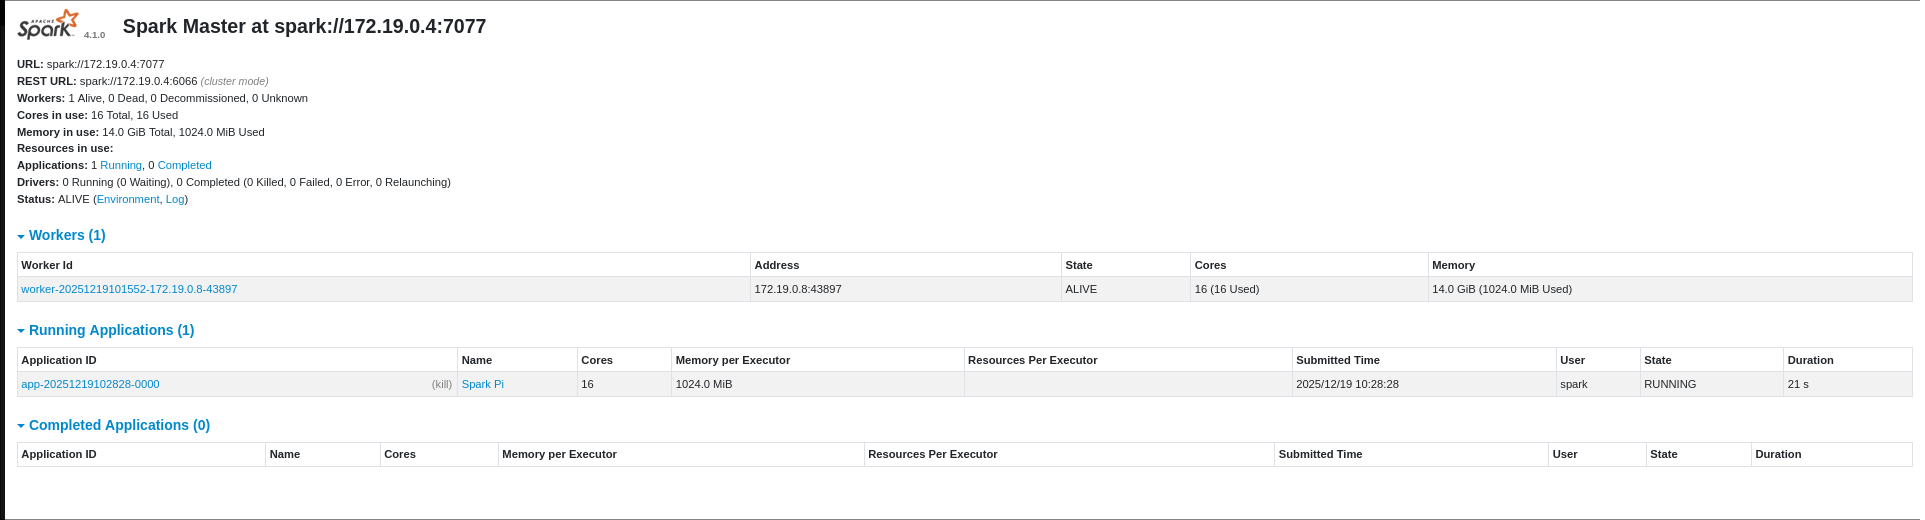
\includegraphics[width=0.78\textwidth]{spark_master_running.png}
    \refstepcounter{figure}
    \caption*{Рисунок \thefigure\ — Spark мастер работает}
    \label{fig:spark_master_running}
\end{figure}

Воркер, выполняющий цикл задач размером 10000, изображен на рисунке \ref{fig:spark_worker_running}

\begin{figure}[H]
    \centering
    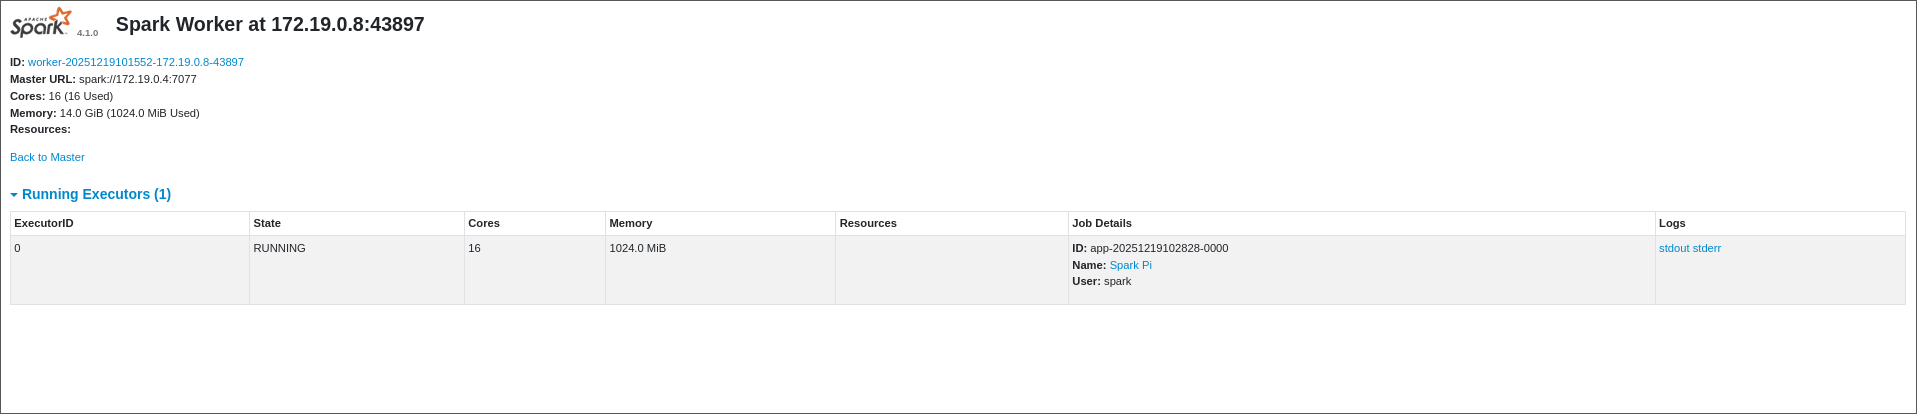
\includegraphics[width=0.78\textwidth]{spark_worker_running.png}
    \refstepcounter{figure}
    \caption*{Рисунок \thefigure\ — Spark воркер работает}
    \label{fig:spark_worker_running}
\end{figure}

Метрики, которые spark\_exporter продуцирует, изображены на рисунке \ref{fig:spark_metrix_raw}

\begin{figure}[H]
    \centering
    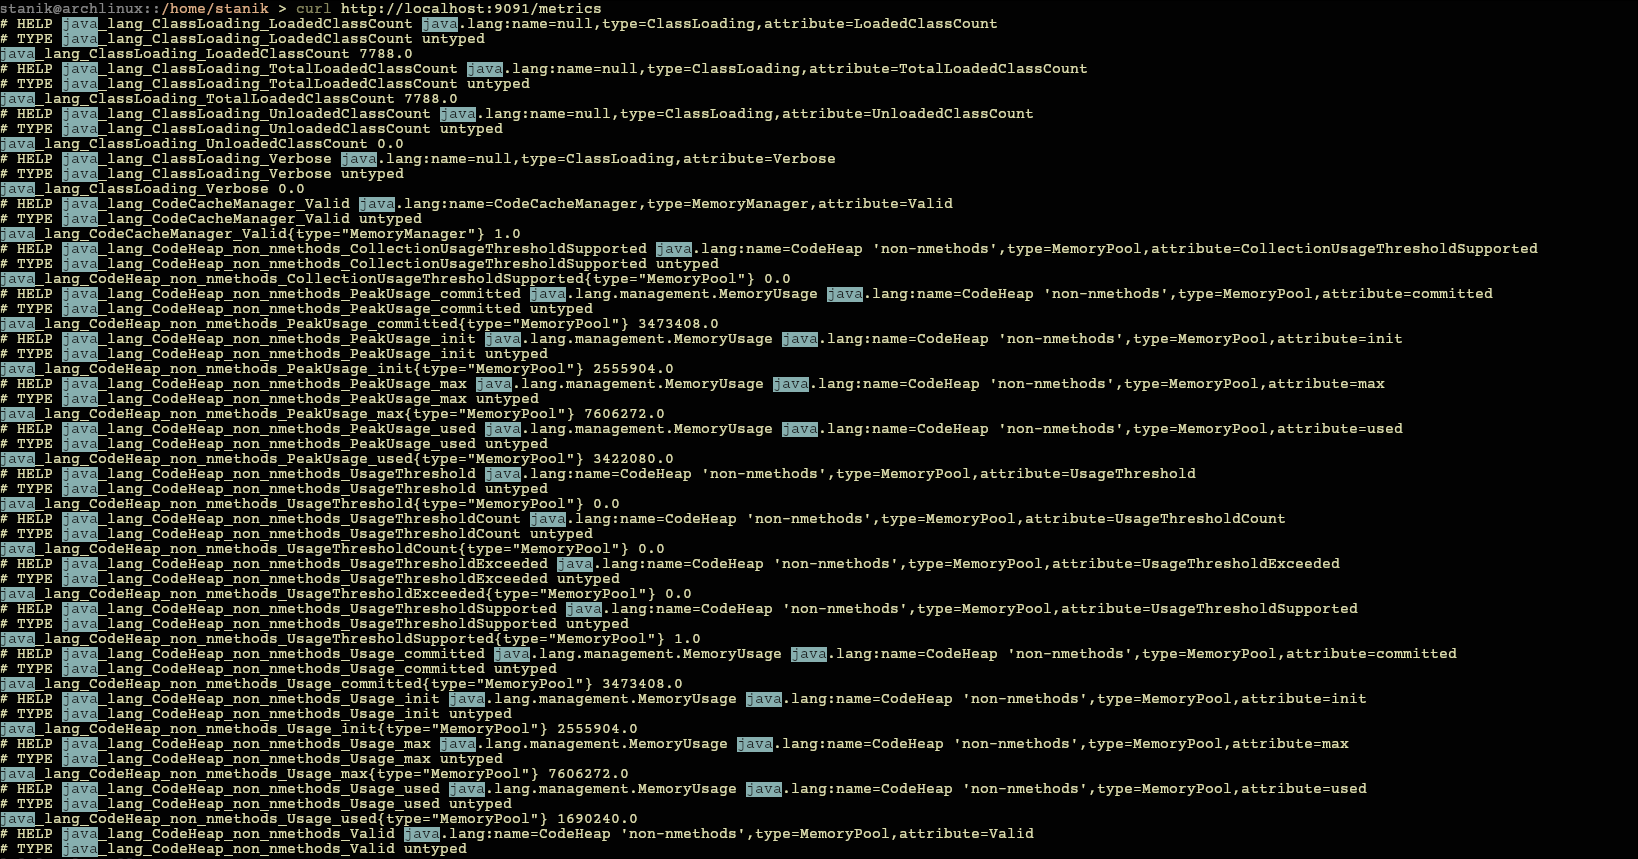
\includegraphics[width=0.78\textwidth]{spark_metrix_raw.png}
    \refstepcounter{figure}
    \caption*{Рисунок \thefigure\ — Spark воркер метрики (сырые)}
    \label{fig:spark_metrix_raw}
\end{figure}

Метрики из spark\_exporter, загруженные в Grafana прямо из Prometheus, изображены на рисунке \ref{fig:spark_metrix_grafana}
\begin{figure}[H]
    \centering
    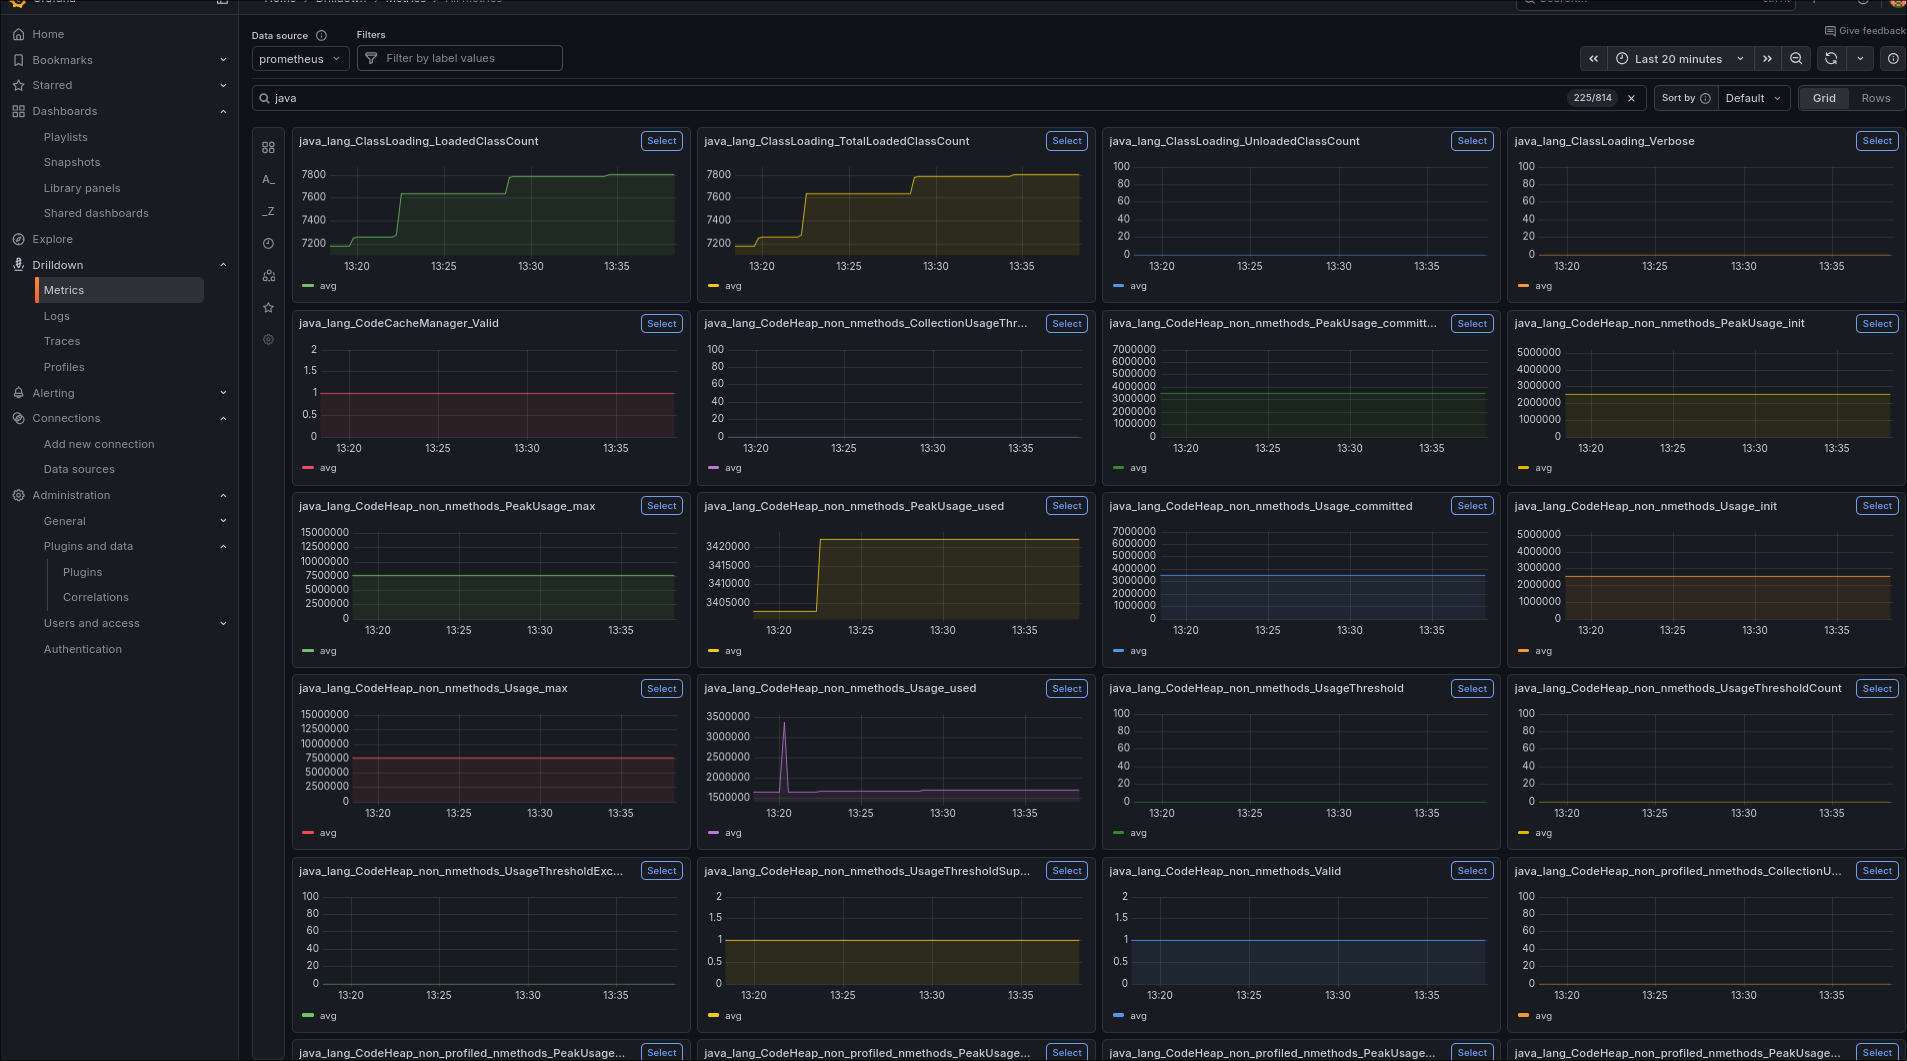
\includegraphics[width=0.78\textwidth]{spark_metrix_grafana.png}
    \refstepcounter{figure}
    \caption*{Рисунок \thefigure\ — Grafana, метрики спарк-воркера}
    \label{fig:spark_metrix_grafana}
\end{figure}

Мастер, завершивший свою задачу, изображен на рисунке \ref{fig:spark_master_finish}

\begin{figure}[H]
    \centering
    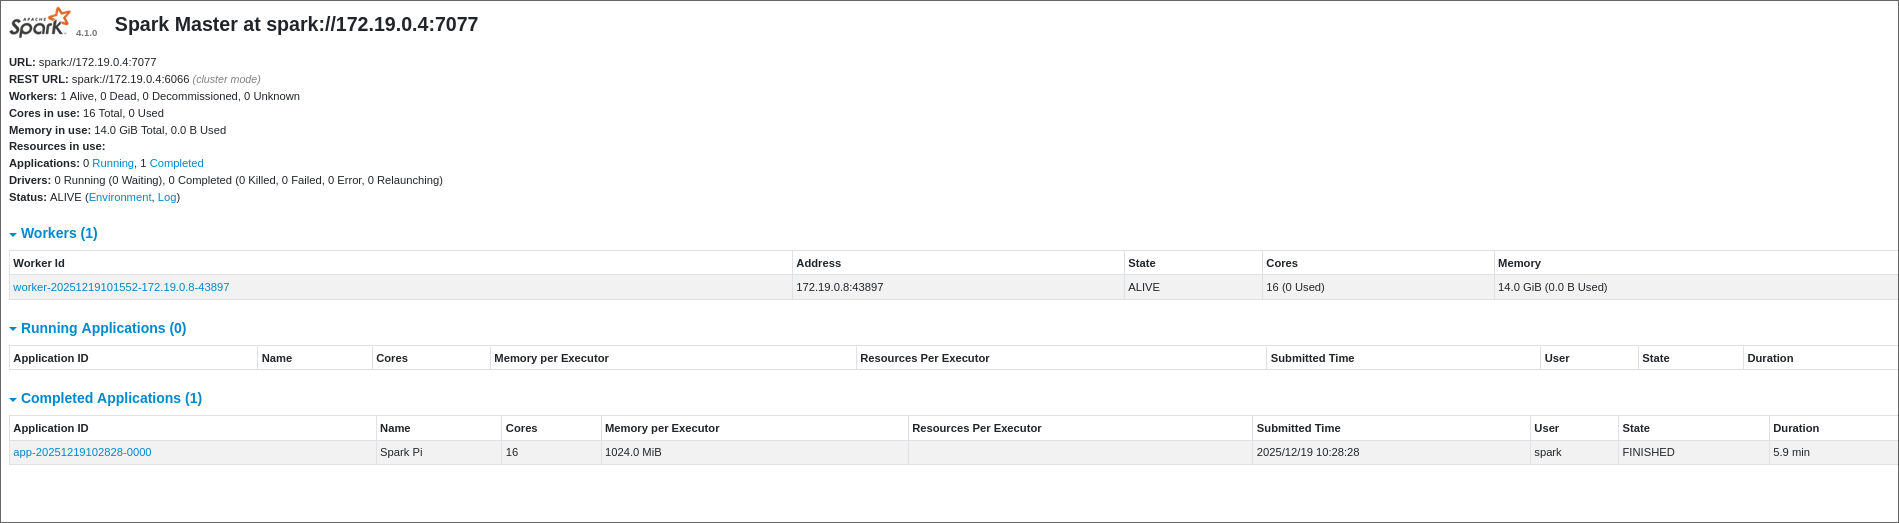
\includegraphics[width=0.78\textwidth]{spark_master_finish.png}
    \refstepcounter{figure}
    \caption*{Рисунок \thefigure\ — Spark мастер завершил выполнение задачи}
    \label{fig:spark_master_finish}
\end{figure}

Воркер, завершивший свою задачу, изображен на рисунке \ref{fig:spark_worker_finish}

\begin{figure}[H]
    \centering
    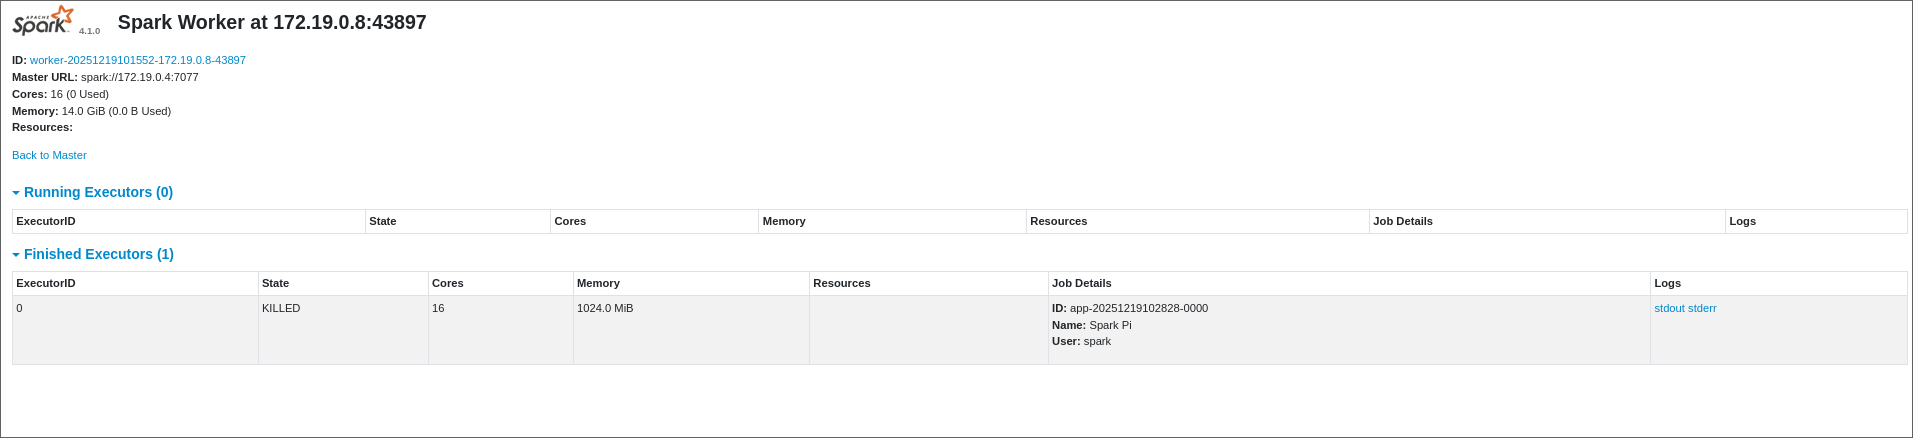
\includegraphics[width=0.78\textwidth]{spark_worker_finish.png}
    \refstepcounter{figure}
    \caption*{Рисунок \thefigure\ — Spark воркер завершил выполнение задачи}
    \label{fig:spark_worker_finish}
\end{figure}

\newpage
\section{Вывод}

В ходе работы была реализована интеграция нескольких технологий для построения
распределённой системы обработки и мониторинга данных. Apache Spark использован
как движок для параллельной обработки больших объёмов данных, обеспечивая
масштабируемое распределение задач между мастер- и воркер-узлами. Apache Kafka
функционирует как система передачи потоковых данных, позволяя надежно
передавать события между источниками и потребителями, при этом обеспечивается
возможность хранения и повторного чтения сообщений. Для визуализации и
мониторинга метрик Spark и состояния потоков данных использованы Prometheus и
Grafana, что обеспечивает наблюдение за производительностью воркеров,
потреблением ресурсов и задержками обработки. Kafdrop добавлен как удобный
веб-интерфейс для наблюдения за состоянием топиков Kafka и их содержимым,
облегчая отладку и тестирование потоковой передачи данных.

Реализованная связка демонстрирует возможности современной распределённой
архитектуры: асинхронная передача данных через Kafka, параллельная обработка в
Spark и комплексный мониторинг с помощью Prometheus и Grafana. Такой подход
позволяет как визуально контролировать нагрузку и использование ресурсов, так и
проводить анализ потоков данных в реальном времени, обеспечивая основу для
построения надёжных систем обработки больших данных и стриминговых приложений.

\newpage
\section{Список источников}

\begin{enumerate}
        \begin{sloppypar}
        \item Apache Spark [Электронный ресурс] /
            Режим доступа к данным: https://spark.apache.org/,
            свободный — 19.12.2025.

        \item Grafana [Электронный ресурс] /
            Режим доступа к данным: https://grafana.com/,
            свободный — 19.12.2025.

        \item Docker [Электронный ресурс] /
            Режим доступа к данным: https://docker.com/,
            свободный — 19.12.2025.

        \item Docker Compose [Электронный ресурс] /
            Режим доступа к данным: https://docs.docker.com/compose/,
            свободный — 19.12.2025.

        \item Docker Images [Электронный ресурс] /
            Режим доступа к данным: https://hub.docker.com/,
            свободный — 19.12.2025.
        \end{sloppypar}
\end{enumerate}

\newpage
\section*{Приложение А. docker\_compose.yml}

\begin{verbatim}

services:
  # spark (master + worker)
  spark-master:
    image: apache/spark:latest
    command: >
      /opt/spark/bin/spark-class
      org.apache.spark.deploy.master.Master
    ports:
      - "7077:7077"
      - "8080:8080"
    networks:
      - spark-net
    environment:
      - SPARK_DAEMON_JAVA_OPTS=
          -Dcom.sun.management.jmxremote
          -Dcom.sun.management.jmxremote.port=7071
          -Dcom.sun.management.jmxremote.rmi.port=7071
          -Dcom.sun.management.jmxremote.authenticate=false
          -Dcom.sun.management.jmxremote.ssl=false
          -Djava.rmi.server.hostname=spark-master

  spark-worker:
    image: apache/spark:latest
    command: >
      /opt/spark/bin/spark-class
      org.apache.spark.deploy.worker.Worker
      spark://spark-master:7077
    depends_on: [spark-master]
    ports:
      - "8081:8081"
    networks:
      - spark-net
    environment:
      - SPARK_DAEMON_JAVA_OPTS=
          -Dcom.sun.management.jmxremote
          -Dcom.sun.management.jmxremote.port=7071
          -Dcom.sun.management.jmxremote.rmi.port=7071
          -Dcom.sun.management.jmxremote.authenticate=false
          -Dcom.sun.management.jmxremote.ssl=false
          -Djava.rmi.server.hostname=spark-worker

  # spark jmx export
  spark-exporter:
    image: bitnami/jmx-exporter:latest
    container_name: spark-exporter
    ports:
      - "9091:9091"
    volumes:
      - ./spark-jmx.yml:/opt/jmx-exporter/config.yml:ro
    command:
      - "9091"
      - "/opt/jmx-exporter/config.yml"
    networks:
      - spark-net

  # kafka + zookeeper + kafdrop
  zookeeper:
    image: confluentinc/cp-zookeeper:7.0.1
    environment:
      ZOOKEEPER_CLIENT_PORT: 2181
      ZOOKEEPER_TICK_TIME: 2000
    ports:
      - "2181:2181"
    networks:
      - spark-net

  kafka:
    image: confluentinc/cp-kafka:7.0.1
    depends_on: [zookeeper]
    ports:
      - "9092:9092"
      - "29092:29092"
    environment:
      KAFKA_BROKER_ID: 1
      KAFKA_ZOOKEEPER_CONNECT: zookeeper:2181
      KAFKA_ADVERTISED_LISTENERS: PLAINTEXT://kafka:29092,PLAINTEXT_HOST://localhost:9092
      KAFKA_LISTENER_SECURITY_PROTOCOL_MAP: PLAINTEXT:PLAINTEXT,PLAINTEXT_HOST:PLAINTEXT
      KAFKA_INTER_BROKER_LISTENER_NAME: PLAINTEXT
      KAFKA_OFFSETS_TOPIC_REPLICATION_FACTOR: 1
    networks:
      - spark-net

  kafdrop:
    image: obsidiandynamics/kafdrop:latest
    depends_on:
      - kafka
    ports:
      - "9009:9009"
    environment:
      KAFKA_BROKER_CONNECT: kafka:29092
      SERVER_PORT: 9009
      JVM_OPTS: "-Xms32M -Xmx64M"
      SERVER_SERVLET_CONTEXTPATH: "/"
    networks:
      - spark-net

  # hadoop
  namenode:
    image: bde2020/hadoop-namenode:2.0.0-hadoop3.2.1-java8
    container_name: namenode
    hostname: namenode
    ports:
      - "9870:9870"  # Web UI
      - "9000:9000"  # RPC port
    environment:
      - CLUSTER_NAME=hadoop-cluster
      - CORE_CONF_fs_defaultFS=hdfs://namenode:9000
    volumes:
      - namenode-data:/hadoop/dfs/name
    restart: unless-stopped

  datanode1:
    image: bde2020/hadoop-datanode:2.0.0-hadoop3.2.1-java8
    container_name: datanode1
    hostname: datanode1
    environment:
      - CORE_CONF_fs_defaultFS=hdfs://namenode:9000
      - HDFS_CONF_dfs__client__use__datanode__hostname=false
    ports:
      - "9864:9864"
    volumes:
      - datanode1-data:/hadoop/dfs/data
    depends_on:
      - namenode
    restart: unless-stopped

  datanode2:
    image: bde2020/hadoop-datanode:2.0.0-hadoop3.2.1-java8
    container_name: datanode2
    hostname: datanode2
    environment:
      - CORE_CONF_fs_defaultFS=hdfs://namenode:9000
      - HDFS_CONF_dfs__client__use__datanode__hostname=false
    volumes:
      - datanode2-data:/hadoop/dfs/data
    depends_on:
      - namenode
    ports:
      - "9865:9864"
    restart: unless-stopped

  # графаня
  prometheus:
    image: prom/prometheus:latest
    container_name: prometheus
    volumes:
      - ./prometheus.yml:/etc/prometheus/prometheus.yml:ro
    ports:
      - "9090:9090"
    command:
      - "--config.file=/etc/prometheus/prometheus.yml"
      - "--storage.tsdb.retention.time=7d"
      - "--web.enable-lifecycle"   # позволяет reload конфигурации
    networks:
      - spark-net

  node_exporter:
    image: prom/node-exporter:latest
    container_name: node_exporter
    ports:
      - "9100:9100"
    networks:
      - spark-net

  grafana:
    image: grafana/grafana:latest
    container_name: grafana
    ports:
      - "3000:3000"
    environment:
      - GF_SECURITY_ADMIN_PASSWORD=admin
    networks:
      - spark-net

volumes:
  namenode-data:
  datanode1-data:
  datanode2-data:

networks:
  spark-net:
    driver: bridge


\end{verbatim}

\newpage
\section*{Приложение Б. prometheus.yml}

\begin{verbatim}

global:
  scrape_interval: 15s
  evaluation_interval: 15s

scrape_configs:
  - job_name: 'prometheus'
    static_configs:
      - targets: ['prometheus:9090']

  - job_name: 'node_exporter'
    static_configs:
      - targets: ['node_exporter:9100']

  - job_name: 'spark'
    static_configs:
      - targets: ['spark-exporter:9091']

\end{verbatim}

\end{document}
